

\clearpage
\begin{figure}
    \centering
    \adddescription{
    \small
This figure plots the cross-sectional distribution of the CECL day-one retained earnings adjustment scaled by pre-adoption equity (percentage points) for community banks at the adoption quarter. The vertical dashed line marks the high-CECL threshold used in the main analysis.
    }
    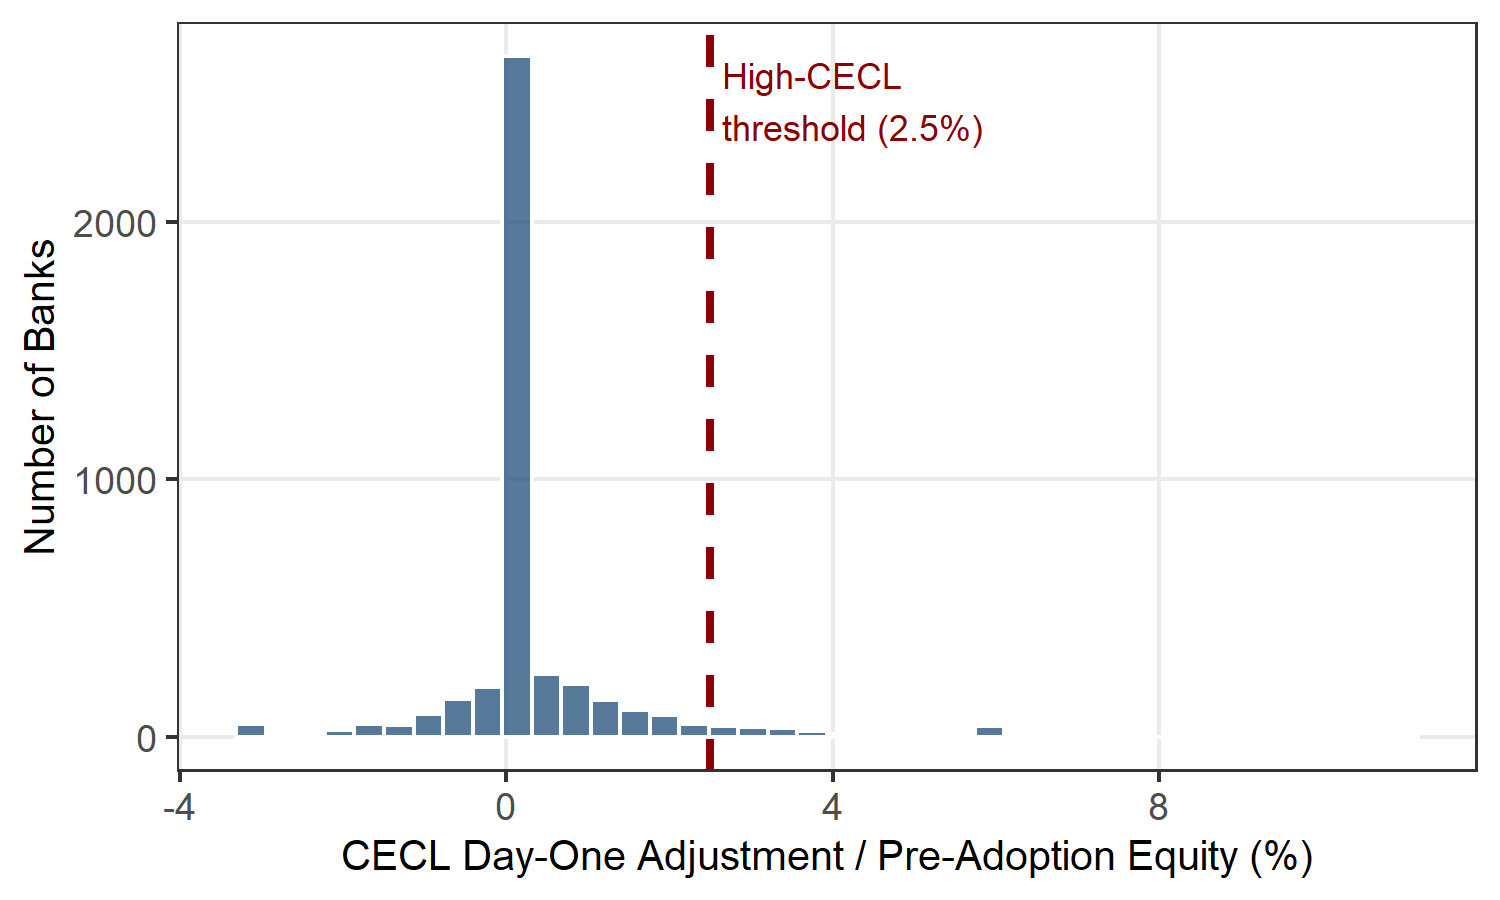
\includegraphics[width=0.75\textwidth]{figures/fig01_cecl_dist_20260403.png}
    \caption{Distribution of CECL adjustment relative to equity}
    \label{fig:cecl_equity_distribution}
\end{figure}


\clearpage
\begin{figure}
    \centering
    \adddescription{
    \small
This figure reports the number of community banks by fiscal quarter of first observed non-missing CECL adjustment in the eligible adoption window. The highlighted bar corresponds to the primary community-bank rollout quarter in the sample construction.
    }
    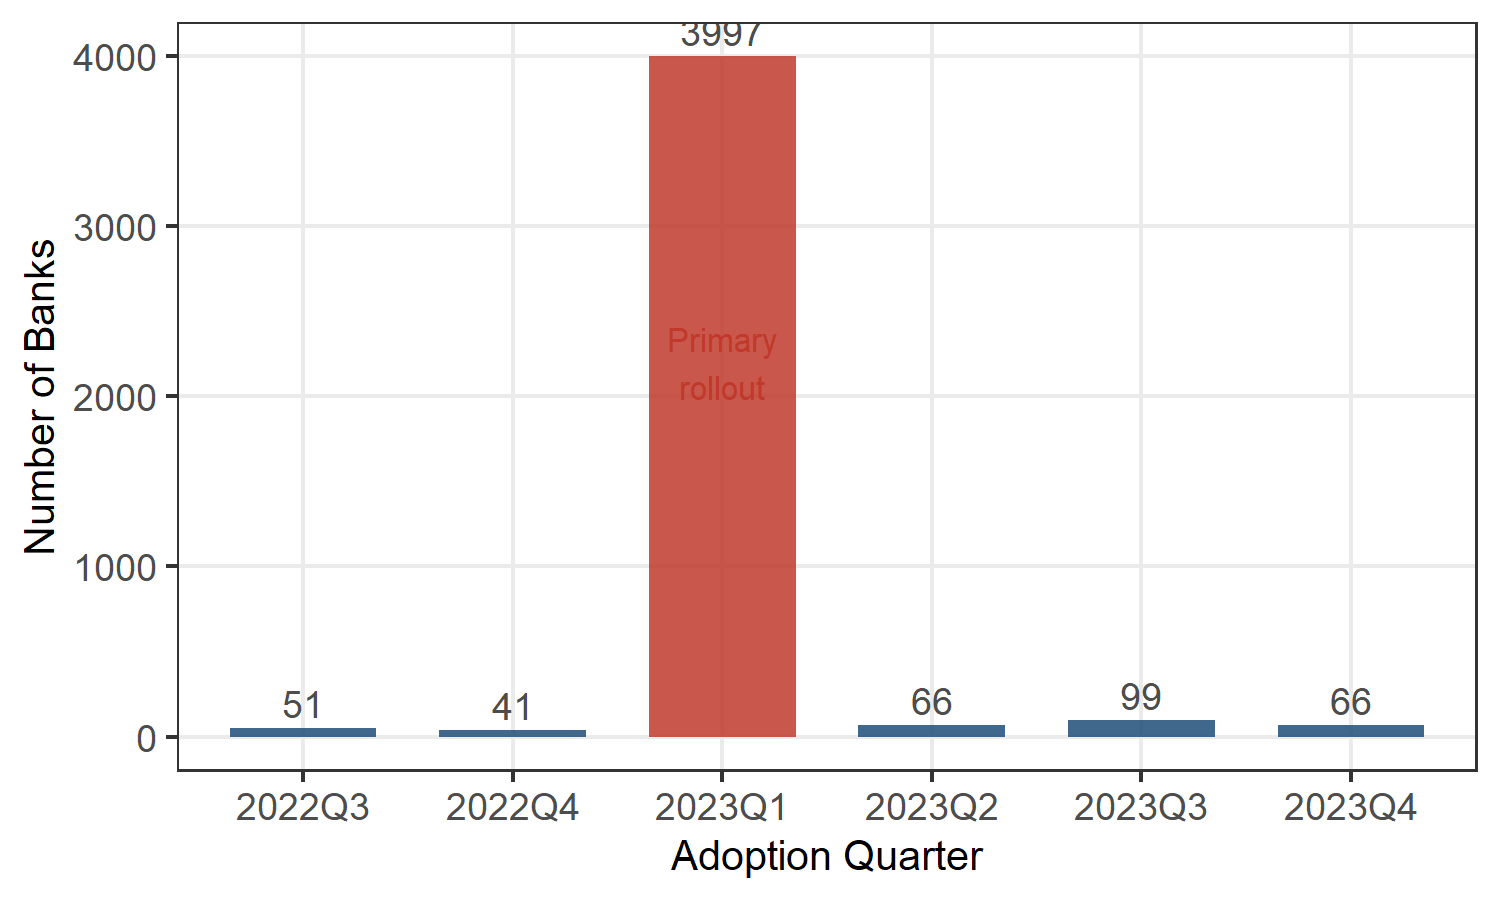
\includegraphics[width=0.75\textwidth]{figures/fig02_adoption_dist_20260403.png}
    \caption{Distribution of CECL adoption quarters}
    \label{fig:cecl_adoption_quarter_distribution}
\end{figure}

\clearpage
\begin{table}[]
    \centering
    \adddescription{
\small
This table reports summary statistics for community banks in the Call Report panel at each bank's CECL adoption quarter among eligible adoption windows. Columns present the full sample, banks with high CECL day-one adjustment relative to pre-adoption equity, and banks with low CECL adjustment, together with the high-minus-low mean difference and two-sample $t$-test significance. Total assets are expressed in millions of dollars; ratio variables are in percentage points. Variables are winsorized at the 1st and 99th percentiles within quarter. The high-CECL indicator uses the project threshold for the continuous adjustment scaled by equity.
    }

    \vspace{0.25cm}
{\small Panel A: Cross-section at adoption quarter}\\
    \resizebox{0.8\textwidth}{!}{
\begingroup
\centering
\begin{tabular}{lrrr rrr rrr r}
  \tabularnewline \midrule \midrule
  & \multicolumn{3}{c}{Full Sample ($N=4320$)} & \multicolumn{3}{c}{High CECL ($N=432$)} & \multicolumn{3}{c}{Low CECL ($N=3888$)} & \\
  \cmidrule(lr){2-4}\cmidrule(lr){5-7}\cmidrule(lr){8-10}
  Variable & Mean & SD & Median & Mean & SD & Median & Mean & SD & Median & Hi$-$Lo \\
  \midrule
  \emph{Balance sheet} & & & & & & & & & & \\
  \hspace{1em}Total Assets (\$M) & 645.991 & 1009.675 & 303.499 & 843.428 & 1152.601 & 413.302 & 624.054 & 990.264 & 296.057 & 219.374*** \\
  \hspace{1em}Equity / Assets (\%) & 10.268 & 8.236 & 8.825 & 9.222 & 3.949 & 8.808 & 10.384 & 8.573 & 8.827 & -1.162*** \\
  \hspace{1em}CECL Adj.\ / Equity (\%) & 0.278 & 1.168 & 0.000 & 2.957 & 1.407 & 2.512 & -0.020 & 0.641 & 0.000 & 2.977*** \\
  \midrule
  \emph{Loan quality} & & & & & & & & & & \\
  \hspace{1em}NPL / Loans (\%) & 0.550 & 0.888 & 0.226 & 0.650 & 0.895 & 0.346 & 0.539 & 0.887 & 0.210 & 0.111** \\
  \hspace{1em}Allowance / Loans (\%) & 1.363 & 0.614 & 1.251 & 1.436 & 0.589 & 1.326 & 1.355 & 0.616 & 1.238 & 0.081*** \\
  \hspace{1em}CRE / Loans (\%) & 25.093 & 16.124 & 23.551 & 26.646 & 14.907 & 26.758 & 24.919 & 16.248 & 23.136 & 1.727** \\
  \midrule
  \emph{Deposit structure} & & & & & & & & & & \\
  \hspace{1em}Unins.\ Time Deps / Assets (\%) & 5.299 & 4.418 & 4.242 & 5.357 & 4.283 & 4.423 & 5.293 & 4.434 & 4.209 & 0.064 \\
  \hspace{1em}Ins.\ Time Deps / Assets (\%) & 7.367 & 5.846 & 5.926 & 8.116 & 6.342 & 6.529 & 7.284 & 5.783 & 5.846 & 0.832*** \\
  \hspace{1em}Unins.\ Deps / Total Deps (\%) & 39.327 & 14.512 & 37.760 & 38.857 & 14.266 & 38.230 & 39.380 & 14.540 & 37.697 & -0.523 \\
  \midrule
  \emph{Performance} & & & & & & & & & & \\
  \hspace{1em}Int.\ Expense / Assets (\%) & 0.230 & 0.136 & 0.210 & 0.253 & 0.140 & 0.227 & 0.227 & 0.135 & 0.208 & 0.026*** \\
  \hspace{1em}ROA (\%) & 0.282 & 0.262 & 0.259 & 0.237 & 0.200 & 0.223 & 0.287 & 0.267 & 0.263 & -0.049*** \\
  \midrule
  \midrule
  \multicolumn{11}{l}{\emph{Cross-section at each bank's CECL adoption quarter. Total assets in \$M.}} \\
  \multicolumn{11}{l}{\emph{Winsorized at 1st/99th percentile by quarter. High CECL $\geq$ 2.5\% of pre-adoption equity.}} \\
  \multicolumn{11}{l}{\emph{Hi$-$Lo: mean difference. Significance: $^{***}$0.01, $^{**}$0.05, $^{*}$0.10 (two-sample $t$-test).}} \\
\end{tabular}
\par\endgroup

    }
    \caption{Summary statistics at CECL adoption}
    \label{tab:descriptive_sumstats_cecl}
\end{table}

\clearpage
\begin{table}[]
    \centering
    \adddescription{
\small
This table reports ordinary least squares estimates of the CECL day-one adjustment scaled by pre-adoption equity (percentage points) on balance-sheet and loan-composition covariates measured at the adoption quarter. Specifications add loan-quality and allowance controls in successive columns. Heteroskedasticity-robust (HC1) standard errors appear in parentheses. *, **, and *** denote statistical significance at the 10\%, 5\%, and 1\% levels, respectively.
    }

    \vspace{0.25cm}
{\small Panel A: Cross-sectional predictors}\\
    \resizebox{0.8\textwidth}{!}{

\begingroup
\centering
\begin{tabular}{lccc}
   \tabularnewline \midrule \midrule
   Dependent Variable: & \multicolumn{3}{c}{CECL Adj}\\
   Model:                           & (1)            & (2)            & (3)\\  
   \midrule
   \emph{Variables}\\
   Constant                         & -0.2871        & -0.5204$^{**}$ & -0.7258$^{***}$\\   
                                    & (0.2054)       & (0.2288)       & (0.2522)\\   
   log(Assets)                      & 0.0457$^{***}$ & 0.0621$^{***}$ & 0.0695$^{***}$\\   
                                    & (0.0159)       & (0.0180)       & (0.0185)\\   
   Equity / Assets (\%)             & -0.0014        & 0.0009         & -0.0035\\   
                                    & (0.0012)       & (0.0030)       & (0.0031)\\   
   NPL / Loans (\%)                 &                & 0.0828$^{***}$ & 0.0642$^{***}$\\   
                                    &                & (0.0235)       & (0.0228)\\   
   CRE / Loans (\%)                 &                & -0.0014        & -0.0018\\   
                                    &                & (0.0011)       & (0.0012)\\   
   C\&I / Loans (\%)                &                & -0.0003        & -0.0018\\   
                                    &                & (0.0021)       & (0.0021)\\   
   Allowance / Loans (\%)           &                &                & 0.1590$^{***}$\\   
                                    &                &                & (0.0367)\\   
   Unrealized Losses / Equity (\%)  &                &                & 0.0008\\   
                                    &                &                & (0.0006)\\   
   \midrule
   \emph{Fit statistics}\\
   Observations                     & 4,320          & 4,252          & 4,243\\  
   Adjusted R$^2$                   & 0.00207        & 0.00537        & 0.01150\\  
   \midrule \midrule
   \multicolumn{4}{l}{\emph{Heteroskedasticity-robust standard-errors in parentheses}}\\
   \multicolumn{4}{l}{\emph{Signif. Codes: ***: 0.01, **: 0.05, *: 0.1}}\\
\end{tabular}
\par\endgroup



    }
    \caption{Predictors of CECL adjustment scaled by equity}
    \label{tab:cecl_predictors_cross_section}
\end{table}

\clearpage
\begin{figure}
    \centering
    \adddescription{
    \small
This figure presents event-study estimates for large banks around CECL day-one adjustment adoption using market-based outcomes. Panel A reports the response of normalized market capitalization, and Panel B reports the response of CDS spreads. The horizontal axis measures months relative to CECL adjustment timing, with month $-1$ omitted as the reference period. Coefficients come from bank and month fixed-effects regressions with log assets as a control and bank-clustered standard errors.
    }
    Panel A: Normalized market cap\\
    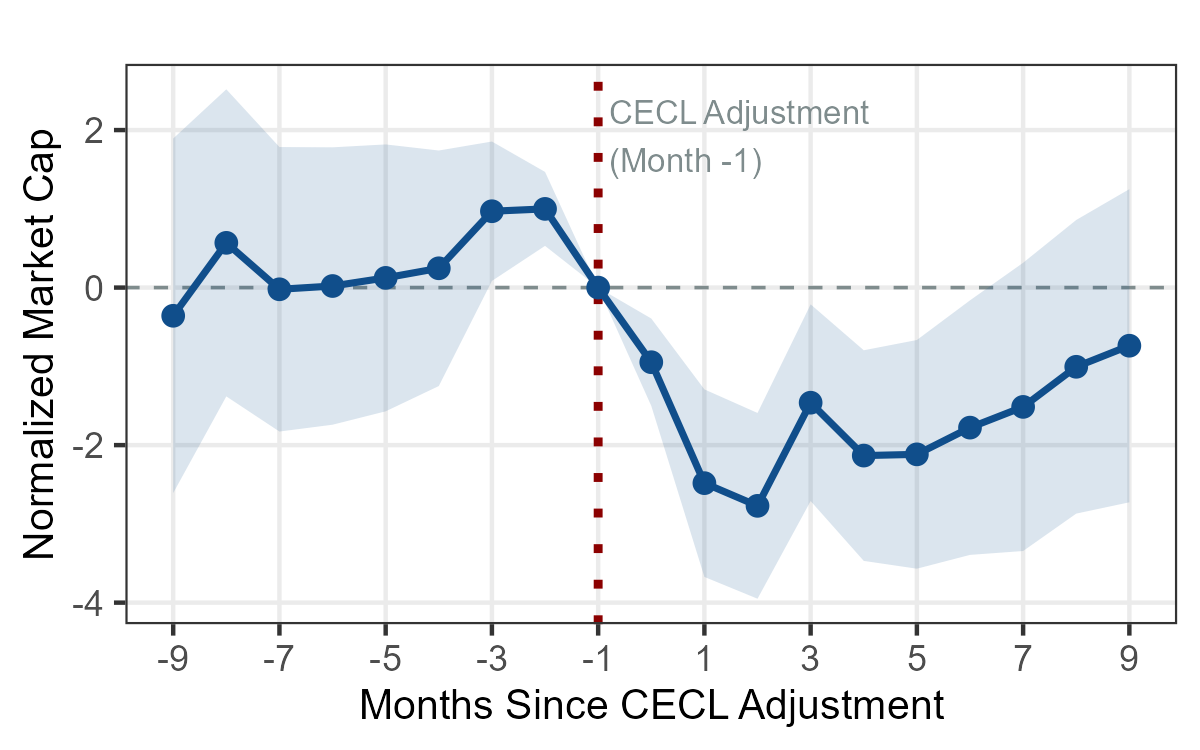
\includegraphics[width=0.75\textwidth]{figures/mkt_cap_large_banks_20260403.png}
    \vspace{0.5cm}\\
    Panel B: CDS spread\\
    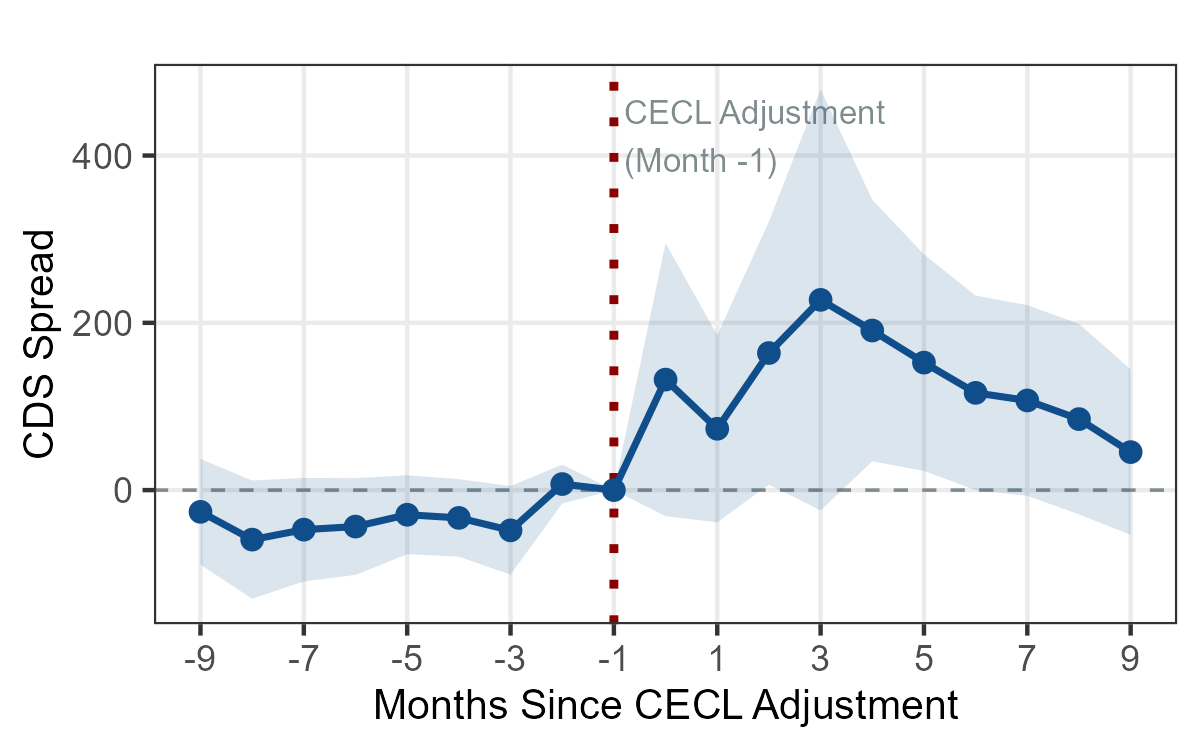
\includegraphics[width=0.75\textwidth]{figures/cds_spread_large_banks_20260403.png}
    \caption{Event-study estimates: market cap and CDS responses for large banks}
    \label{fig:es_large_banks_market_cds}
\end{figure}

\clearpage
\begin{table}[]
    \centering
    \adddescription{
\small
This table reports bank-by-quarter difference-in-differences estimates for community banks in the Call Report panel. The dependent variables are uninsured time deposits scaled by assets (columns 1--2) and insured time deposits scaled by assets (columns 3--4), each expressed in percentage points. Columns (1) and (3) include an interaction of a post-2023Q1 indicator with the continuous CECL day-one adjustment relative to equity; columns (2) and (4) include an interaction of the post indicator with an indicator for high CECL exposure (top decile). All specifications include bank and quarter fixed effects, lagged log assets, lagged equity-to-assets ratio, and lagged interest expense to assets. Standard errors are clustered at the bank level. *, **, and *** denote statistical significance at the 10\%, 5\%, and 1\% levels, respectively.
    }

    \vspace{0.25cm}
{\small Panel A: Community banks}\\
    \resizebox{0.8\textwidth}{!}{

\begingroup
\centering
\begin{tabular}{lcccc}
   \tabularnewline \midrule \midrule
   Dependent Variables: & \multicolumn{2}{c}{Unins. Time Dep./Assets (\%)} & \multicolumn{2}{c}{Ins. Time Dep./Assets (\%)}\\
   Model:                         & (1)             & (2)             & (3)             & (4)\\  
   \midrule
   \emph{Variables}\\
   Post x CECL Adj                & -0.0724$^{**}$  &                 & 0.0699          &   \\   
                                  & (0.0357)        &                 & (0.0509)        &   \\   
   Post x High CECL               &                 & -0.3935$^{**}$  &                 & 0.7117$^{**}$\\   
                                  &                 & (0.1815)        &                 & (0.2905)\\   
   Post                           & 0.0576          & 0.0552          & -0.1525         & -0.1659\\   
                                  & (0.0920)        & (0.0915)        & (0.1160)        & (0.1159)\\   
   log(Assets), $t{-}1$           & -0.3484         & -0.3559         & 0.1700          & 0.1664\\   
                                  & (0.2366)        & (0.2358)        & (0.3154)        & (0.3137)\\   
   Equity/Assets (\%), $t{-}1$    & -0.0555$^{***}$ & -0.0558$^{***}$ & -0.0873$^{***}$ & -0.0870$^{***}$\\   
                                  & (0.0114)        & (0.0114)        & (0.0195)        & (0.0195)\\   
   Int. Exp/Assets (\%), $t{-}1$  & 5.042$^{***}$   & 5.043$^{***}$   & 6.334$^{***}$   & 6.315$^{***}$\\   
                                  & (0.3096)        & (0.3100)        & (0.4131)        & (0.4129)\\   
   \midrule
   \emph{Fixed-effects}\\
   Bank                           & Yes             & Yes             & Yes             & Yes\\  
   Quarter                        & Yes             & Yes             & Yes             & Yes\\  
   \midrule
   \emph{Fit statistics}\\
   Observations                   & 97,064          & 97,064          & 97,064          & 97,064\\  
   Adjusted R$^2$                 & 0.82123         & 0.82123         & 0.86398         & 0.86410\\  
   \midrule \midrule
   \multicolumn{5}{l}{\emph{Clustered (Bank) standard-errors in parentheses}}\\
   \multicolumn{5}{l}{\emph{Signif. Codes: ***: 0.01, **: 0.05, *: 0.1}}\\
\end{tabular}
\par\endgroup



    }
    \caption{Difference-in-differences: time deposits and CECL exposure}
    \label{tab:small_bank_did_time_deposits}
\end{table}






\clearpage
\begin{figure}
    \centering
    \adddescription{
    \small
This figure plots event-study estimates for community banks in the quarterly Call Report panel. The horizontal axis measures quarters relative to CECL adoption ($k=0$ corresponds to 2023Q1 for community banks). The top row uses uninsured time deposits scaled by assets as the outcome; the bottom row uses insured time deposits scaled by assets. The left column reports coefficients on leads and lags of high CECL exposure interacted with quarter indicators; the right column reports coefficients on leads and lags of the continuous CECL day-one adjustment relative to equity interacted with quarter indicators. In each specification $k=-1$ is omitted; the vertical axis is the estimated coefficient and the shaded band is a pointwise 90\% confidence interval. Standard errors are clustered at the bank level.
    }
    {\small Uninsured time deposits / assets}\\[0.25em]
    \begin{minipage}[t]{0.48\textwidth}
        \centering
        {\small High CECL}\\[-0.25em]
        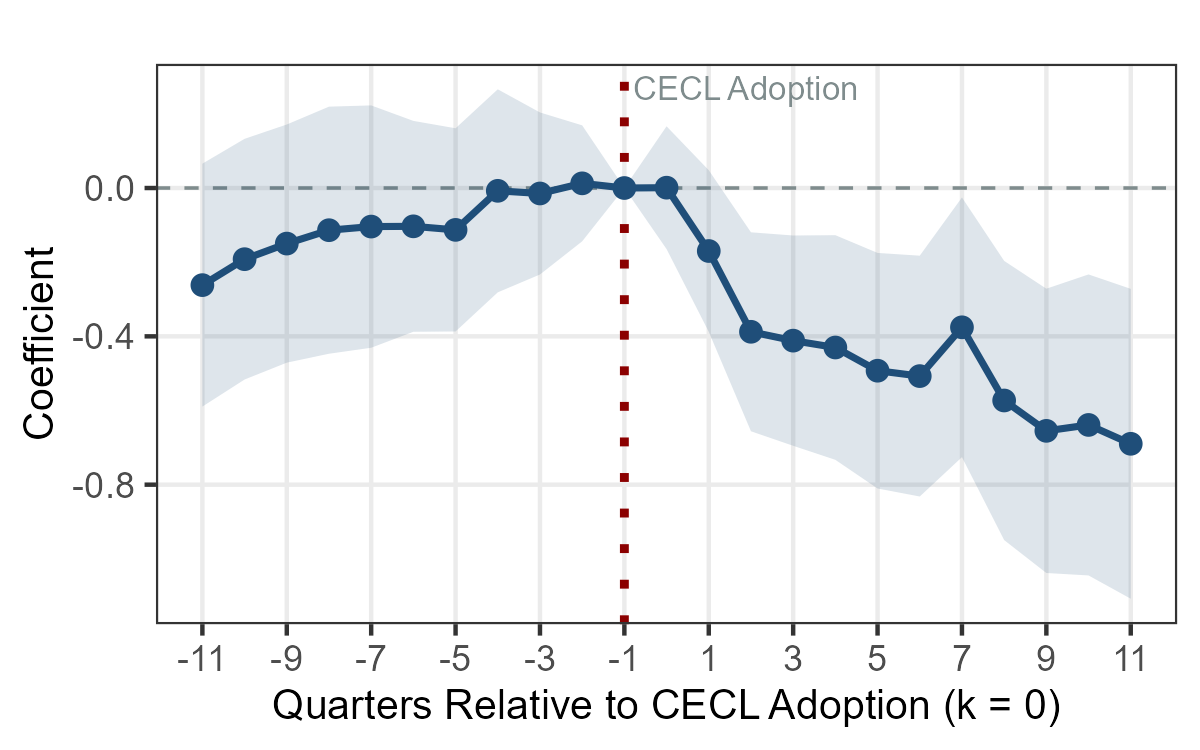
\includegraphics[width=\linewidth]{figures/es_unins_time_deps_assets_20260403.png}
    \end{minipage}\hfill
    \begin{minipage}[t]{0.48\textwidth}
        \centering
        {\small Continuous CECL adj.}\\[-0.25em]
        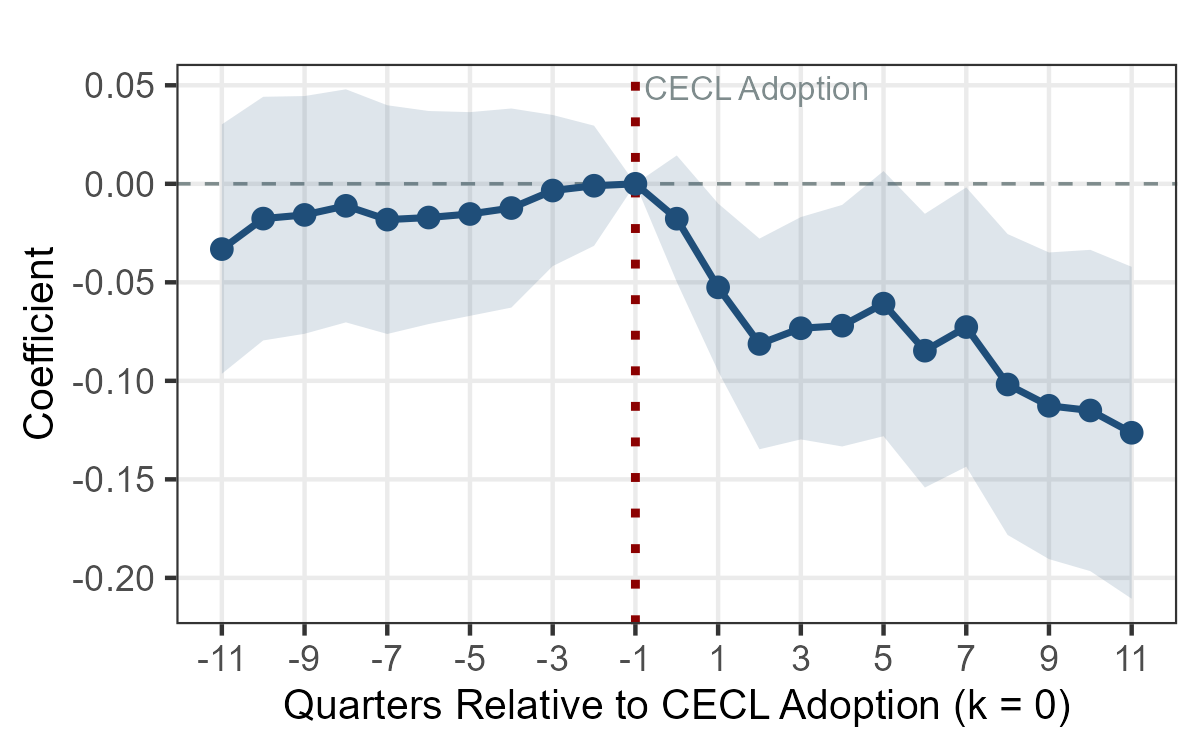
\includegraphics[width=\linewidth]{figures/es_unins_time_deps_assets_cecl_cont_20260403.png}
    \end{minipage}
    \vspace{0.5cm}\\
    {\small Insured time deposits / assets}\\[0.25em]
    \begin{minipage}[t]{0.48\textwidth}
        \centering
        {\small High CECL}\\[-0.25em]
        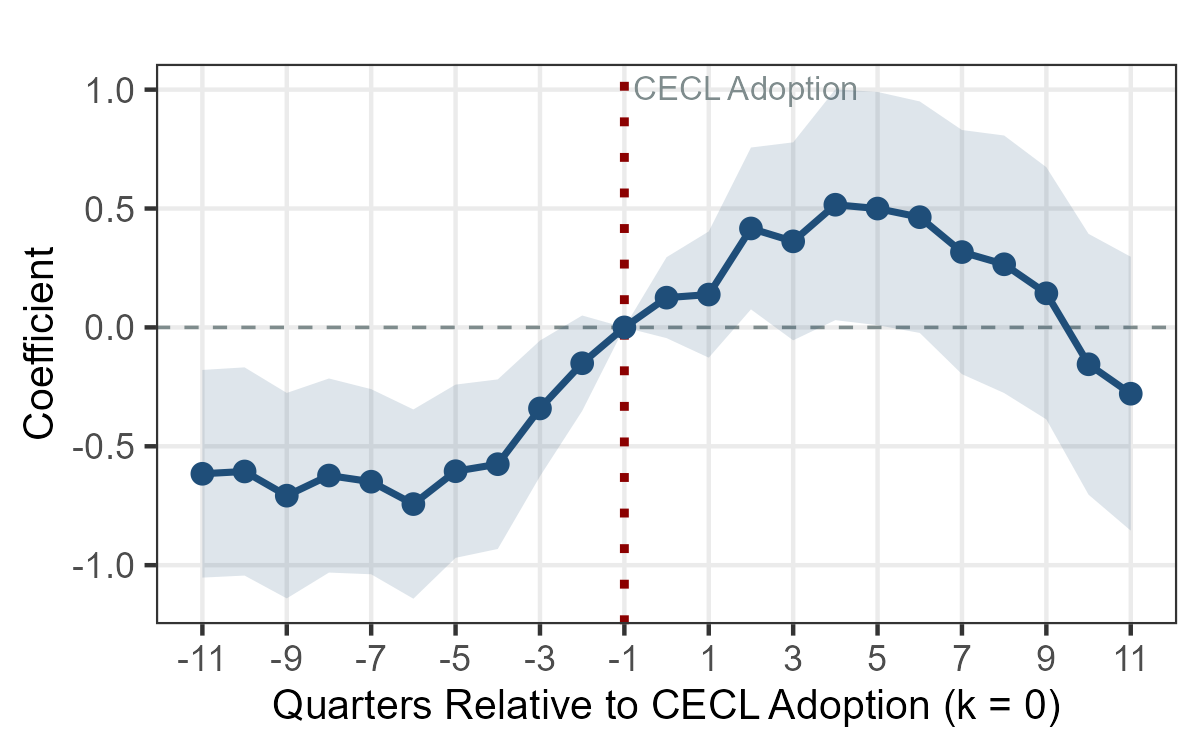
\includegraphics[width=\linewidth]{figures/es_ins_time_deps_assets_20260403.png}
    \end{minipage}\hfill
    \begin{minipage}[t]{0.48\textwidth}
        \centering
        {\small Continuous CECL adj.}\\[-0.25em]
        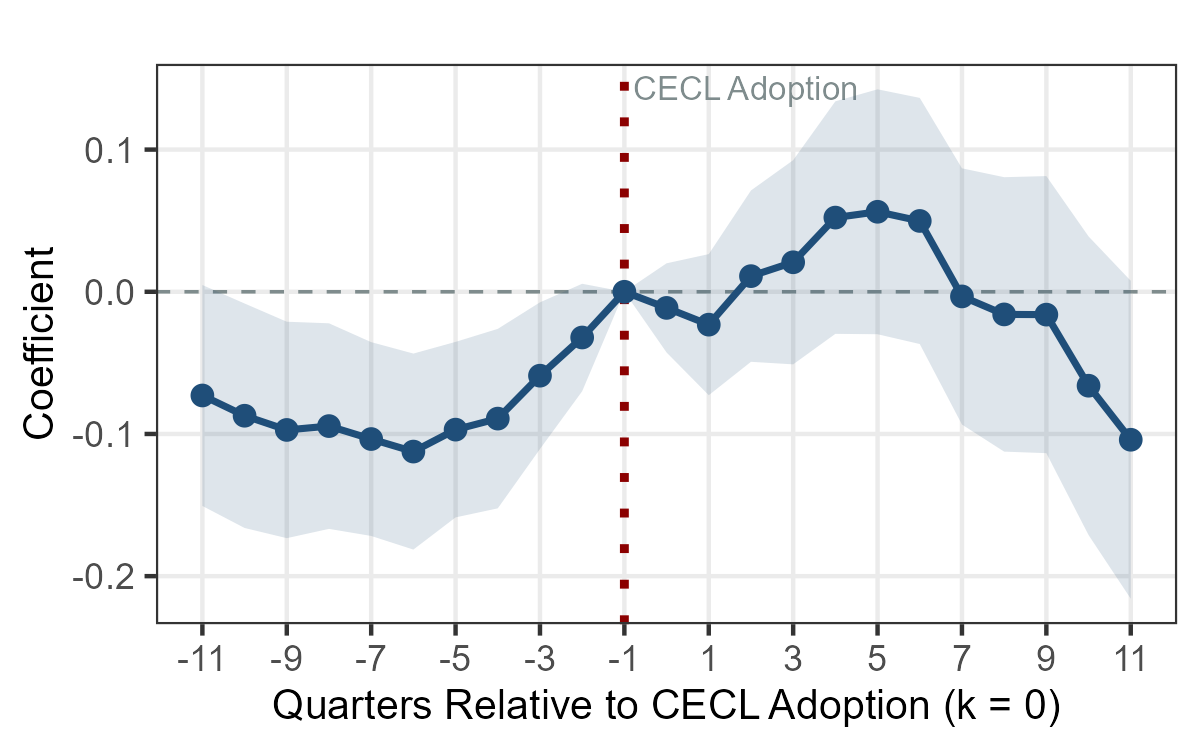
\includegraphics[width=\linewidth]{figures/es_ins_time_deps_assets_cecl_cont_20260403.png}
    \end{minipage}
    \caption{Event-study estimates: time deposits around CECL adoption}
    \label{fig:es_time_deps_cecl}
\end{figure}

\clearpage
\begin{table}[]
    \centering
    \adddescription{
\small
This table reports triple-difference estimates for community banks using a stacked bank-by-quarter panel in which each row corresponds to either uninsured or insured time deposits scaled by assets (percentage points), with an indicator for the uninsured deposit series. Column (1) includes two-way interactions of the post-2023Q1 indicator and the continuous CECL day-one adjustment relative to equity with the uninsured indicator, as well as the corresponding triple interaction; column (2) uses an indicator for high CECL exposure (top decile) in place of the continuous adjustment. All specifications include bank $\times$ quarter fixed effects. Standard errors are clustered at the bank level. *, **, and *** denote statistical significance at the 10\%, 5\%, and 1\% levels, respectively.
    }

    \vspace{0.25cm}
{\small Panel A: Community banks}\\
    \resizebox{0.8\textwidth}{!}{

\begingroup
\centering
\begin{tabular}{lcc}
   \tabularnewline \midrule \midrule
   Dependent Variable: & \multicolumn{2}{c}{Deposits/Assets (\%)}\\
   Model:                                                & (1)             & (2)\\  
   \midrule
   \emph{Variables}\\
   Uninsured time dep                                    & -2.825$^{***}$  & -2.835$^{***}$\\   
                                                         & (0.0793)        & (0.0788)\\   
   CECL Adj $\times$ Uninsured time dep                  & -0.2113$^{***}$ &   \\   
                                                         & (0.0707)        &   \\   
   Post $\times$ Uninsured time dep                      & 0.8855$^{***}$  & 0.8981$^{***}$\\   
                                                         & (0.0637)        & (0.0637)\\   
   CECL Adj $\times$ Post $\times$ Uninsured time dep    & -0.1770$^{***}$ &   \\   
                                                         & (0.0578)        &   \\   
   High CECL $\times$ Uninsured time dep                 &                 & -0.9769$^{***}$\\   
                                                         &                 & (0.3656)\\   
   High CECL $\times$ Post $\times$ Uninsured time dep   &                 & -1.252$^{***}$\\   
                                                         &                 & (0.3401)\\   
   \midrule
   \emph{Fixed-effects}\\
   Bank x Quarter                                        & Yes             & Yes\\  
   \midrule
   \emph{Fit statistics}\\
   Observations                                          & 194,128         & 194,128\\  
   Adjusted R$^2$                                        & 0.44489         & 0.44499\\  
   \midrule \midrule
   \multicolumn{3}{l}{\emph{Clustered (Bank) standard-errors in parentheses}}\\
   \multicolumn{3}{l}{\emph{Signif. Codes: ***: 0.01, **: 0.05, *: 0.1}}\\
\end{tabular}
\par\endgroup



    }
    \caption{Triple difference: time deposits, CECL, and uninsured status}
    \label{tab:small_bank_triple_diff_time_deposits}
\end{table}



\clearpage
\begin{table}[]
    \centering
    \adddescription{
\small
This table reports bank-by-quarter difference-in-differences estimates for community banks in the Call Report panel. The dependent variables are interest expense scaled by assets (columns 1--2), return on assets (columns 3--4), and net interest margin (columns 5--6), each expressed in percentage points where applicable. Odd columns include an interaction of a post-2023Q1 indicator with the continuous CECL day-one adjustment relative to equity; even columns include an interaction of the post indicator with an indicator for high CECL exposure (top decile). All specifications include bank and quarter fixed effects, lagged log assets, and lagged equity-to-assets ratio. Standard errors are clustered at the bank level. *, **, and *** denote statistical significance at the 10\%, 5\%, and 1\% levels, respectively.
    }

    \vspace{0.25cm}
{\small Panel A: Community banks}\\
    \resizebox{0.8\textwidth}{!}{

\begingroup
\centering
\begin{tabular}{lcccccc}
   \tabularnewline \midrule \midrule
   Dependent Variables: & \multicolumn{2}{c}{Int. Exp/Assets (\%)} & \multicolumn{2}{c}{ROA (\%)} & \multicolumn{2}{c}{NIM/Assets (\%)}\\
   Model:                       & (1)            & (2)            & (3)                   & (4)             & (5)            & (6)\\  
   \midrule
   \emph{Variables}\\
   Post x CECL Adj              & 0.0037$^{**}$  &                & -0.0088$^{***}$       &                 & -0.0047$^{**}$ &   \\   
                                & (0.0015)       &                & (0.0021)              &                 & (0.0018)       &   \\   
   Post x High CECL             &                & 0.0214$^{***}$ &                       & -0.0378$^{***}$ &                & -0.0235$^{**}$\\   
                                &                & (0.0079)       &                       & (0.0105)        &                & (0.0098)\\   
   Post                         & 0.0069$^{*}$   & 0.0070$^{*}$   & $5.45\times 10^{-5}$  & -0.0007         & 0.0107         & 0.0104\\   
                                & (0.0041)       & (0.0041)       & (0.0083)              & (0.0083)        & (0.0068)       & (0.0068)\\   
   log(Assets), $t{-}1$         & 0.1974$^{***}$ & 0.1977$^{***}$ & 0.0384$^{***}$        & 0.0371$^{**}$   & -0.0296$^{*}$  & -0.0301$^{*}$\\   
                                & (0.0139)       & (0.0139)       & (0.0145)              & (0.0145)        & (0.0169)       & (0.0169)\\   
   Equity/Assets (\%), $t{-}1$  & 0.0003         & 0.0003         & -0.0012               & -0.0012         & 0.0074$^{***}$ & 0.0074$^{***}$\\   
                                & (0.0005)       & (0.0005)       & (0.0013)              & (0.0013)        & (0.0010)       & (0.0010)\\   
   \midrule
   \emph{Fixed-effects}\\
   Bank                         & Yes            & Yes            & Yes                   & Yes             & Yes            & Yes\\  
   Quarter                      & Yes            & Yes            & Yes                   & Yes             & Yes            & Yes\\  
   \midrule
   \emph{Fit statistics}\\
   Observations                 & 97,084         & 97,084         & 97,084                & 97,084          & 97,084         & 97,084\\  
   Adjusted R$^2$               & 0.88558        & 0.88559        & 0.60300               & 0.60288         & 0.70081        & 0.70078\\  
   \midrule \midrule
   \multicolumn{7}{l}{\emph{Clustered (Bank) standard-errors in parentheses}}\\
   \multicolumn{7}{l}{\emph{Signif. Codes: ***: 0.01, **: 0.05, *: 0.1}}\\
\end{tabular}
\par\endgroup



    }
    \caption{Difference-in-differences: financial outcomes and CECL exposure}
    \label{tab:small_bank_did_financial_outcomes}
\end{table}

\clearpage
\begin{figure}
    \centering
    \adddescription{
    \small
This figure plots event-study estimates for community banks in the quarterly Call Report panel. The horizontal axis measures quarters relative to CECL adoption ($k=0$ corresponds to 2023Q1 for community banks). Each row corresponds to a different dependent variable: interest expense scaled by assets, return on assets, and net interest margin. The left column reports coefficients on leads and lags of high CECL exposure interacted with quarter indicators; the right column reports coefficients on leads and lags of the continuous CECL day-one adjustment relative to equity interacted with quarter indicators. In each specification $k=-1$ is omitted; the vertical axis is the estimated coefficient and the shaded band is a pointwise 90\% confidence interval. Standard errors are clustered at the bank level.
    }
    {\small Interest expense / assets}\\[0.25em]
    \begin{minipage}[t]{0.48\textwidth}
        \centering
        {\small High CECL}\\[-0.25em]
        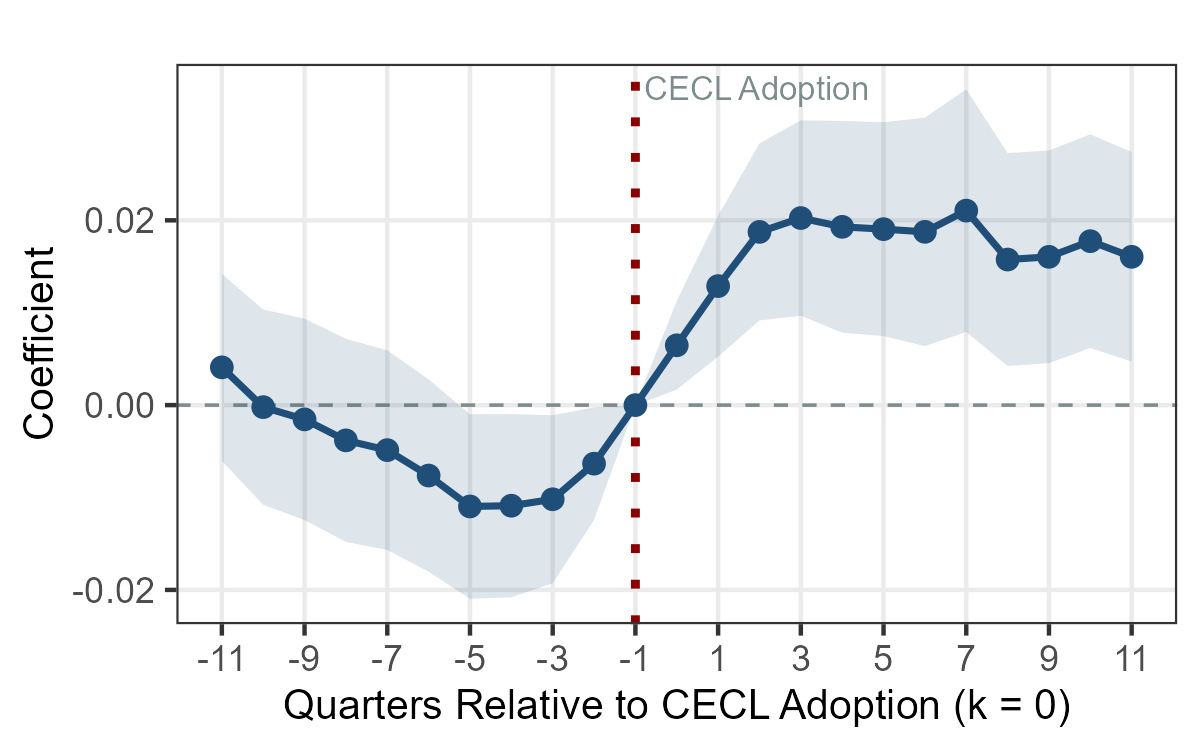
\includegraphics[width=\linewidth]{figures/es_int_expense_assets_20260403.png}
    \end{minipage}\hfill
    \begin{minipage}[t]{0.48\textwidth}
        \centering
        {\small Continuous CECL adj.}\\[-0.25em]
        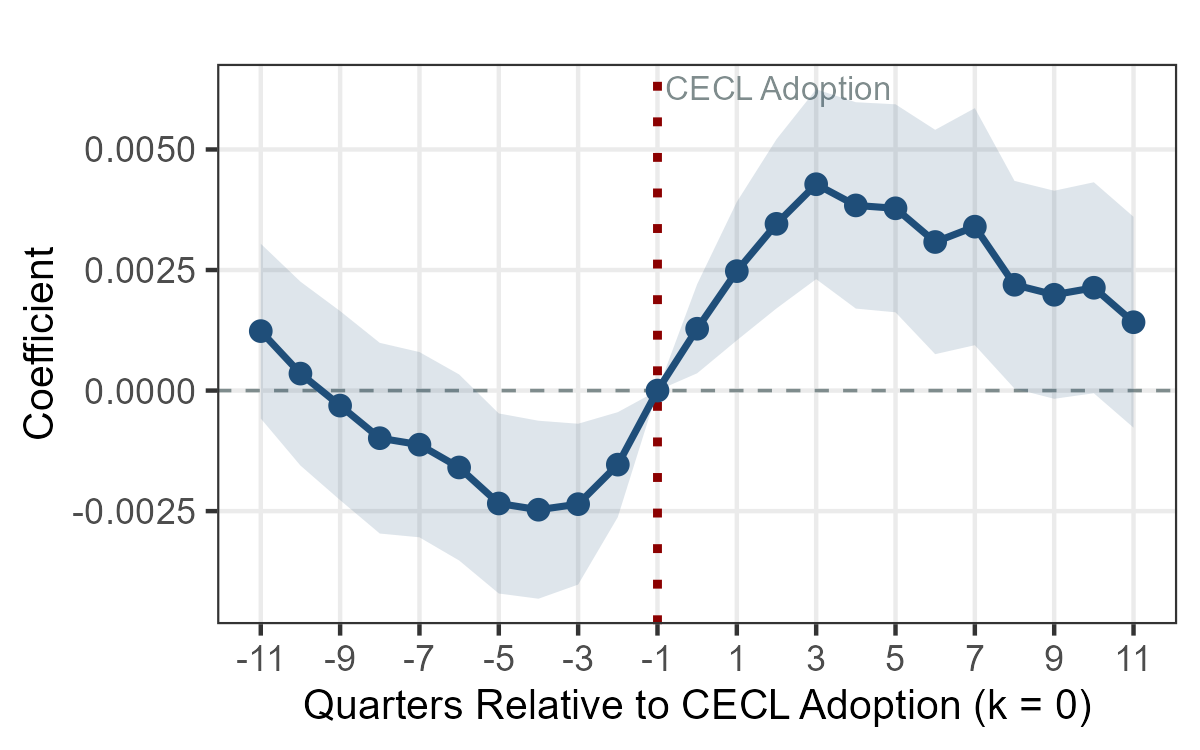
\includegraphics[width=\linewidth]{figures/es_int_expense_assets_cecl_cont_20260403.png}
    \end{minipage}
    \vspace{0.5cm}\\
    {\small Return on assets}\\[0.25em]
    \begin{minipage}[t]{0.48\textwidth}
        \centering
        {\small High CECL}\\[-0.25em]
        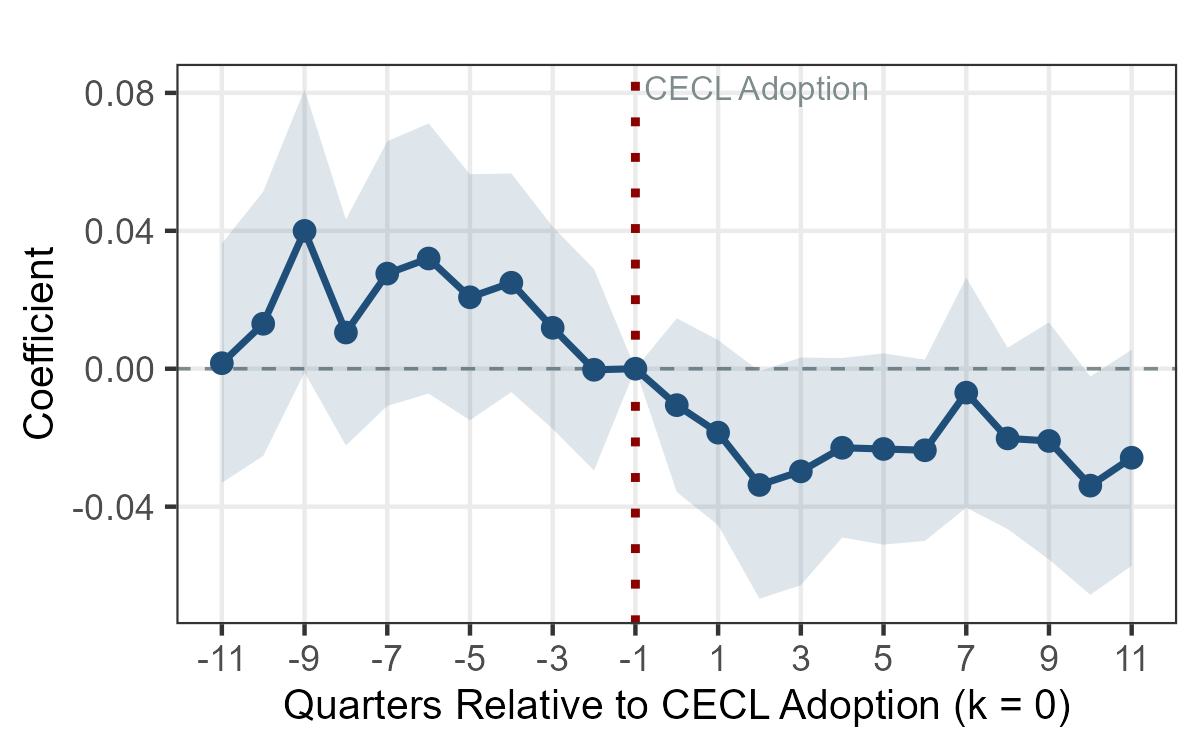
\includegraphics[width=\linewidth]{figures/es_roa_20260403.png}
    \end{minipage}\hfill
    \begin{minipage}[t]{0.48\textwidth}
        \centering
        {\small Continuous CECL adj.}\\[-0.25em]
        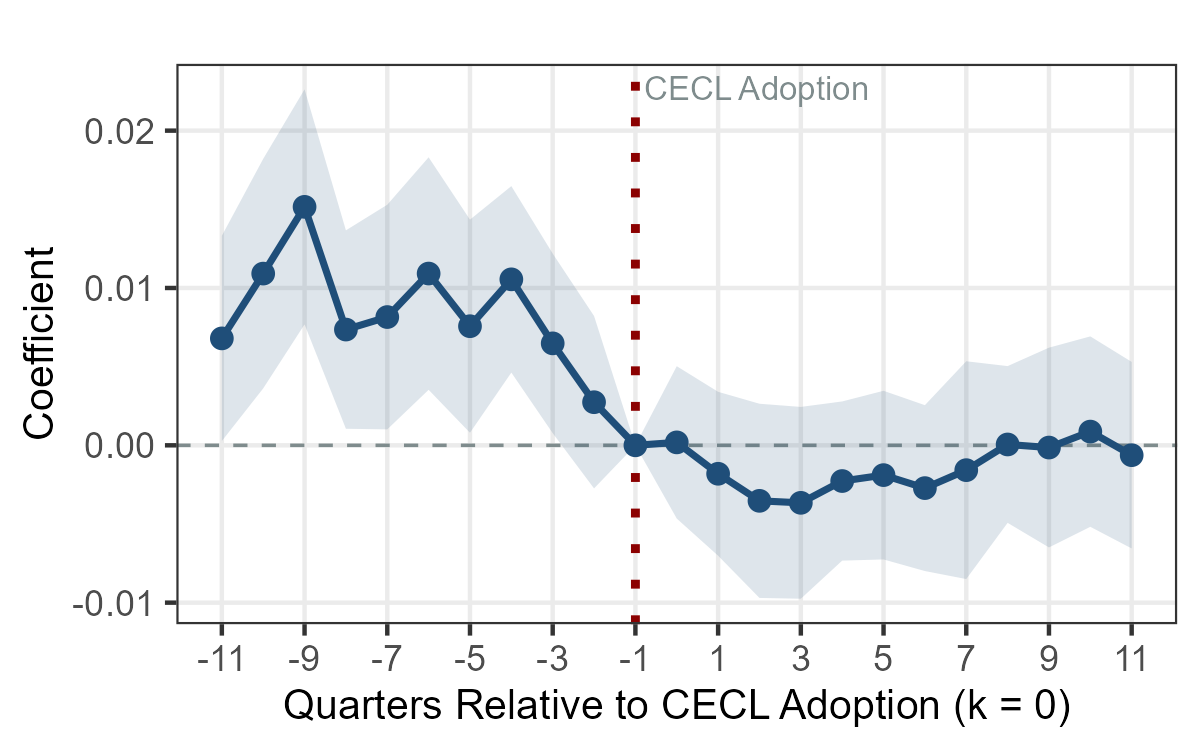
\includegraphics[width=\linewidth]{figures/es_roa_cecl_cont_20260403.png}
    \end{minipage}
    \vspace{0.5cm}\\
    {\small Net interest margin}\\[0.25em]
    \begin{minipage}[t]{0.48\textwidth}
        \centering
        {\small High CECL}\\[-0.25em]
        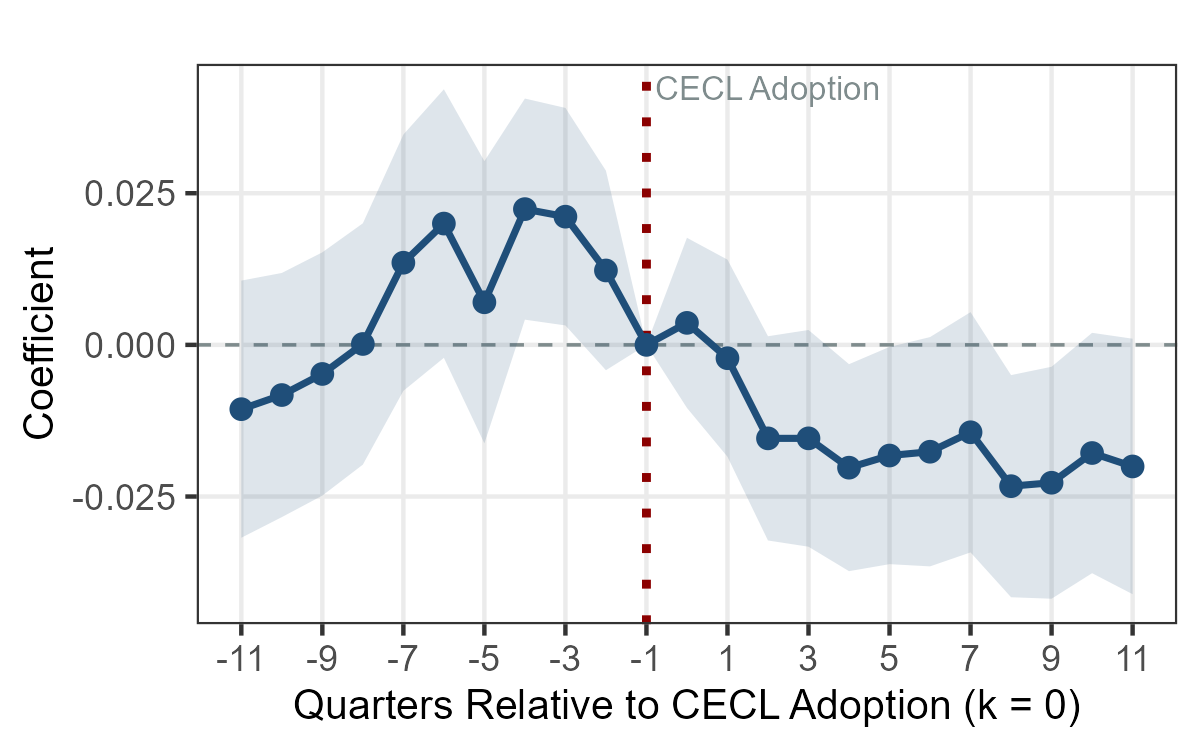
\includegraphics[width=\linewidth]{figures/es_nim_20260403.png}
    \end{minipage}\hfill
    \begin{minipage}[t]{0.48\textwidth}
        \centering
        {\small Continuous CECL adj.}\\[-0.25em]
        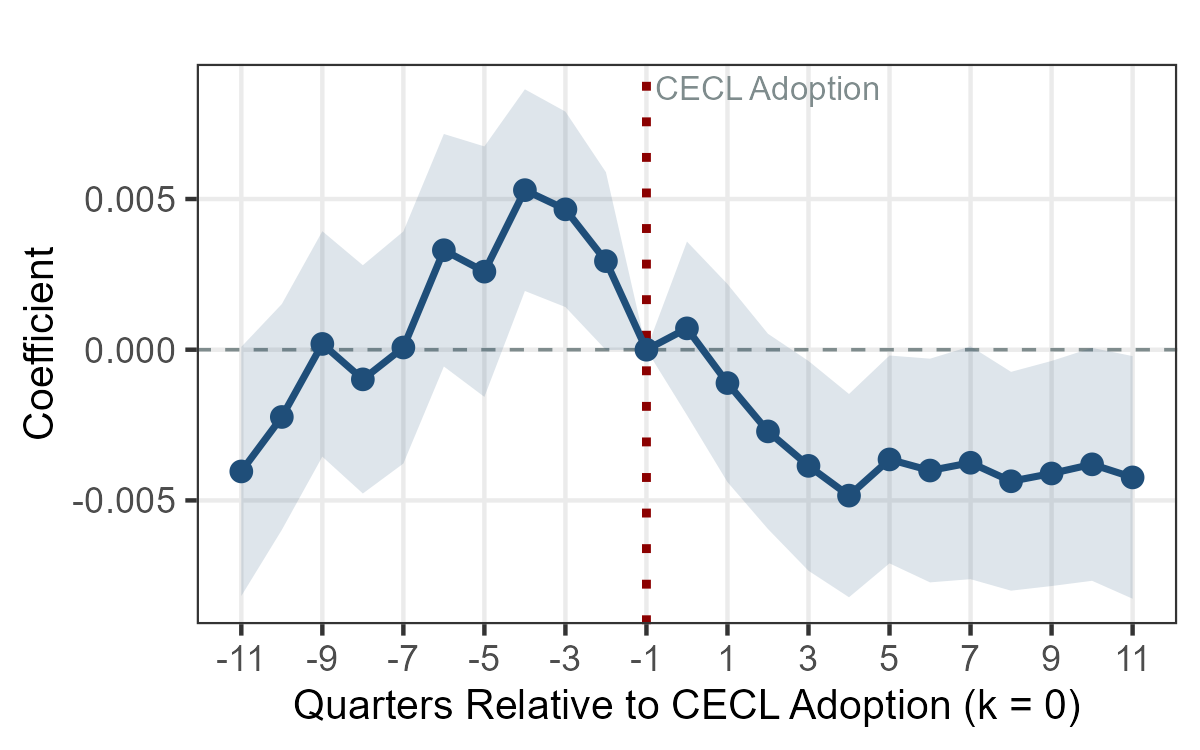
\includegraphics[width=\linewidth]{figures/es_nim_cecl_cont_20260403.png}
    \end{minipage}
    \caption{Event-study estimates: financial outcomes around CECL adoption}
    \label{fig:es_financial_outcomes_cecl}
\end{figure}


\clearpage
\begin{figure}
    \centering
    \adddescription{
    \small
This figure presents event-study estimates by depositor sophistication for community banks in the quarterly Call Report panel. The horizontal axis measures quarters relative to CECL adoption, with $k=-1$ as the omitted reference period. Each panel reports one dependent variable and overlays estimates for high- and low-sophistication banks. All specifications include bank and calendar-quarter fixed effects, lagged controls consistent with the corresponding table specification, and bank-clustered standard errors. The note printed below each panel reports the estimated Post $\times$ High CECL $\times$ High Sophistication coefficient and standard error from the associated triple-interaction regression.
    }
    \begin{minipage}[t]{0.48\textwidth}
        \centering
        {\small Panel A: Uninsured time deposits / assets}\\[-0.25em]
        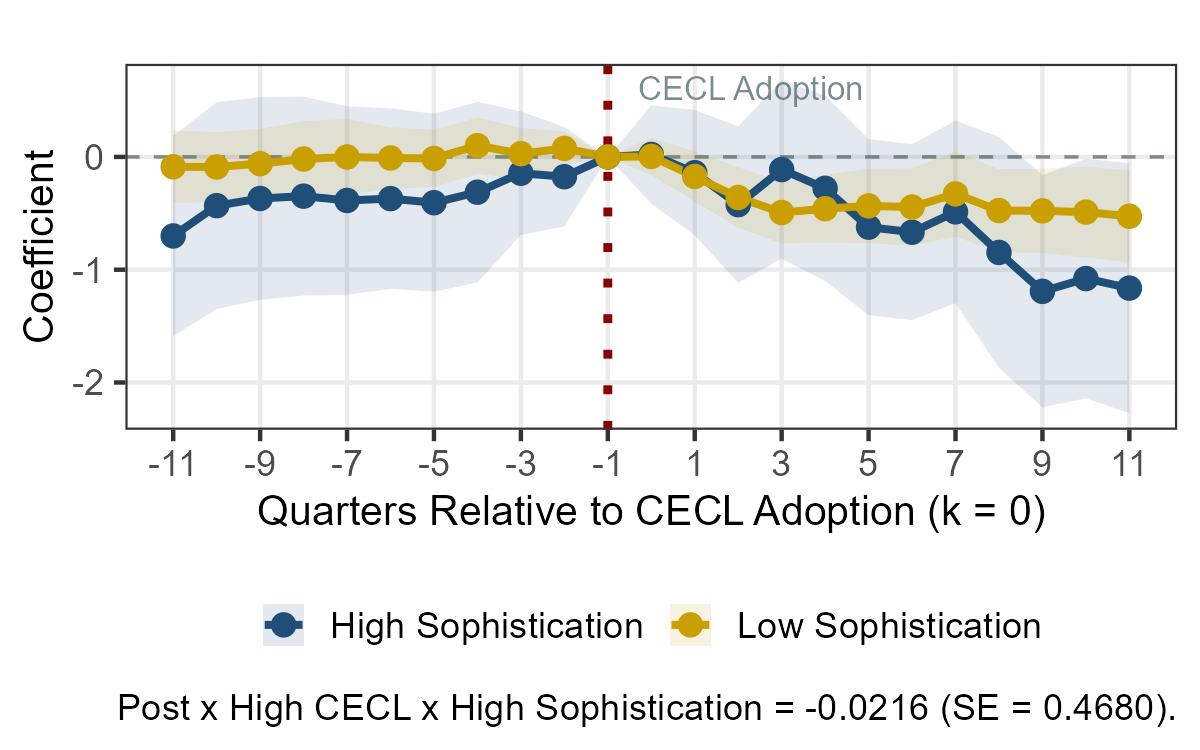
\includegraphics[width=\linewidth]{figures/es_soph_split_unins_time_deps_assets_20260403.png}
    \end{minipage}\hfill
    \begin{minipage}[t]{0.48\textwidth}
        \centering
        {\small Panel B: Insured time deposits / assets}\\[-0.25em]
        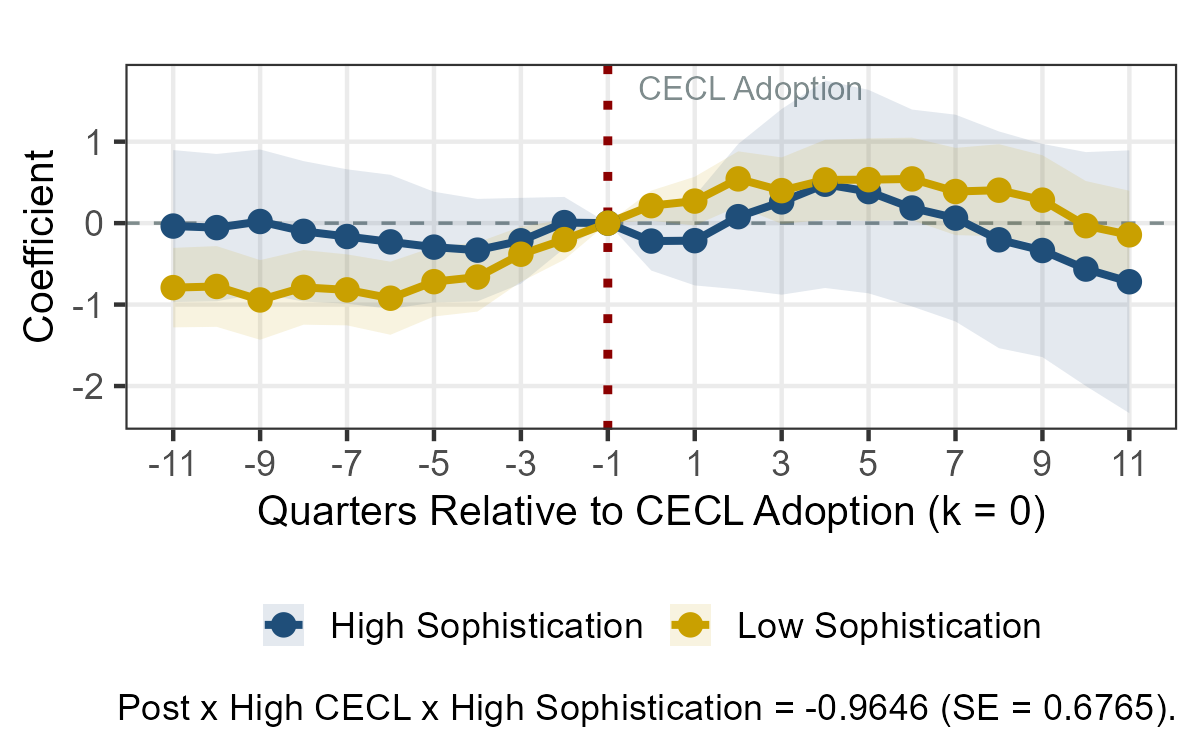
\includegraphics[width=\linewidth]{figures/es_soph_split_ins_time_deps_assets_20260403.png}
    \end{minipage}
    \vspace{0.5cm}\\
    \begin{minipage}[t]{0.48\textwidth}
        \centering
        {\small Panel C: Interest expense / assets}\\[-0.25em]
        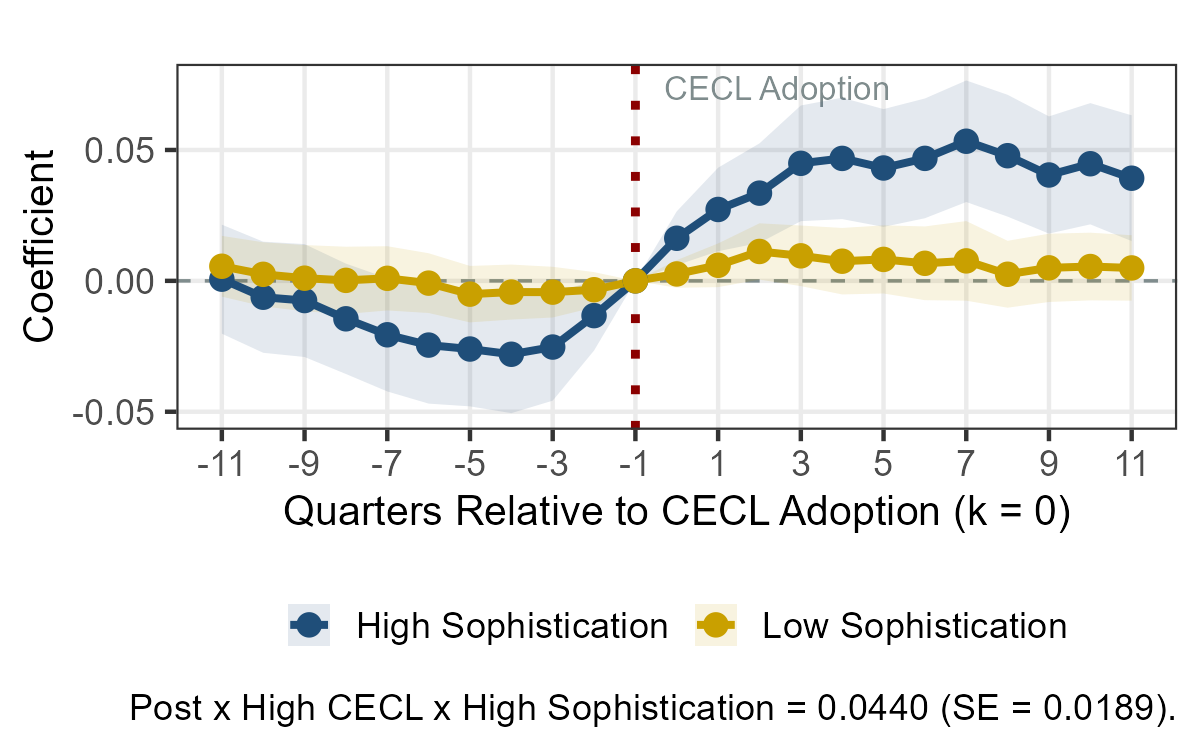
\includegraphics[width=\linewidth]{figures/es_soph_split_int_expense_assets_20260403.png}
    \end{minipage}\hfill
    \begin{minipage}[t]{0.48\textwidth}
        \centering
        {\small Panel D: Return on assets}\\[-0.25em]
        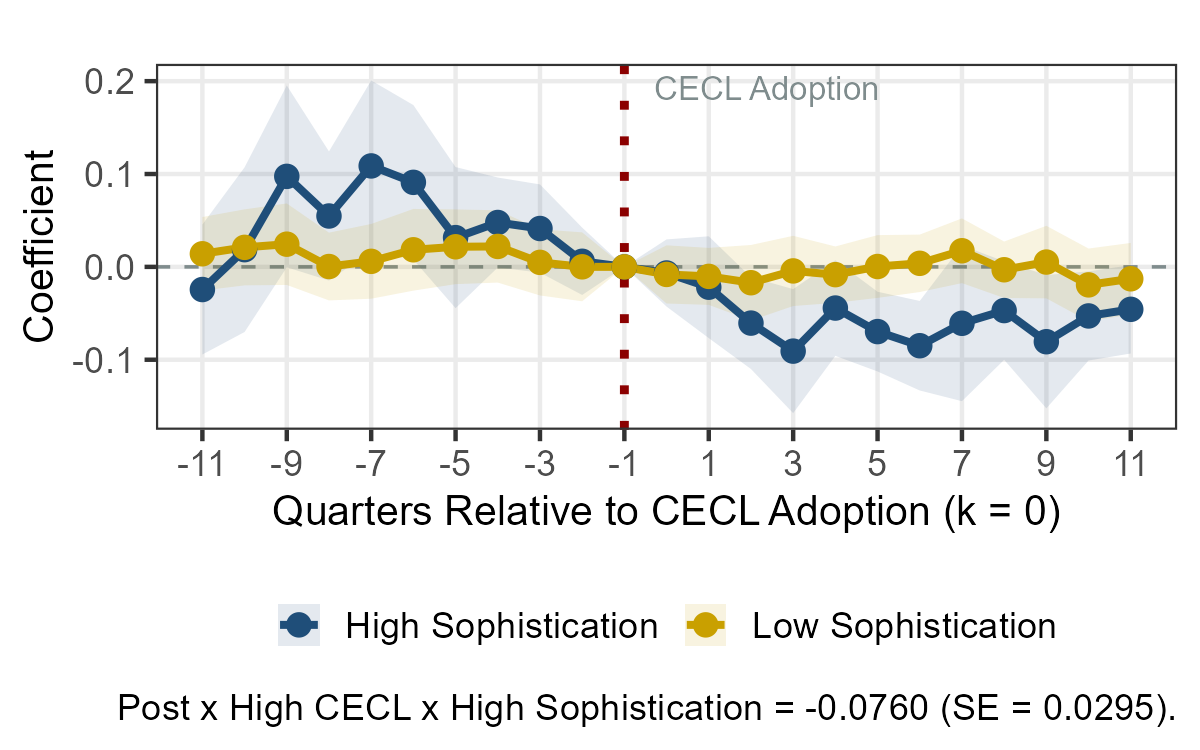
\includegraphics[width=\linewidth]{figures/es_soph_split_roa_20260403.png}
    \end{minipage}
    \vspace{0.5cm}\\
    \begin{minipage}[t]{0.65\textwidth}
        \centering
        {\small Panel E: Net interest margin / assets}\\[-0.25em]
        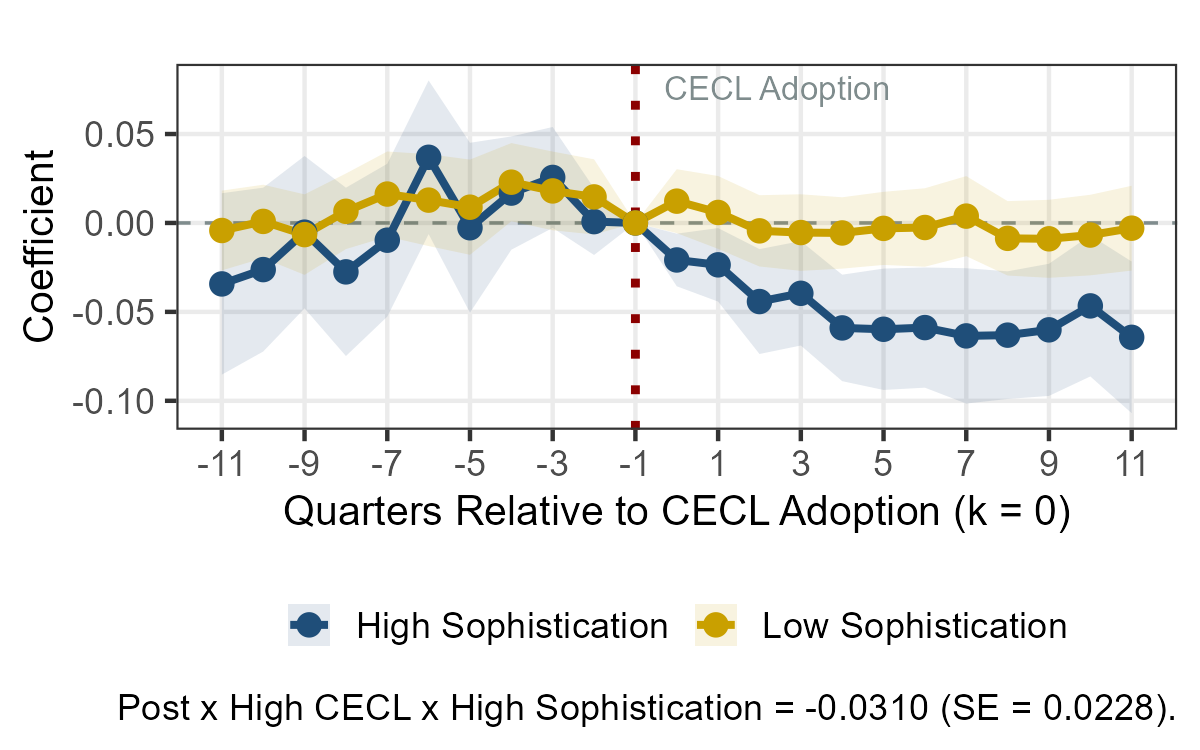
\includegraphics[width=\linewidth]{figures/es_soph_split_nim_20260403.png}
    \end{minipage}
    \caption{Event-study estimates by depositor sophistication}
    \label{fig:es_sophistication_split}
\end{figure}
